\begin{table}[h]
    \centering
    \renewcommand{\arraystretch}{1.3}  % Adjust row height
    \begin{tabular}{|c|c|c|}
        \hline
        \textbf{Component} & \textbf{ATmega328P Pin} & \textbf{Connection Description} \\
        \hline
        BCD Input A & Digital Pin 2 & Connected to 7447 A input \\
        BCD Input B & Digital Pin 3 & Connected to 7447 B input \\
        BCD Input C & Digital Pin 4 & Connected to 7447 C input \\
        BCD Input D & Digital Pin 5 & Connected to 7447 D input \\
        \hline
        COM (Tens Place) & Analog Pin A3 (PC3) & Common pin for 7-segment (Tens) \\
        COM (Units Place) & Analog Pin A4 (PC4) & Common pin for 7-segment (Units) \\
        \hline
        7-Segment Display & 7447 Output & 7447 drives segments \\
        \hline
    \end{tabular}
    \vspace{0.5cm}
    \caption{Pin Connections for 7-Segment Display with 7447 and ATmega328P}
\end{table}
\begin{figure}[H]
    \centering
    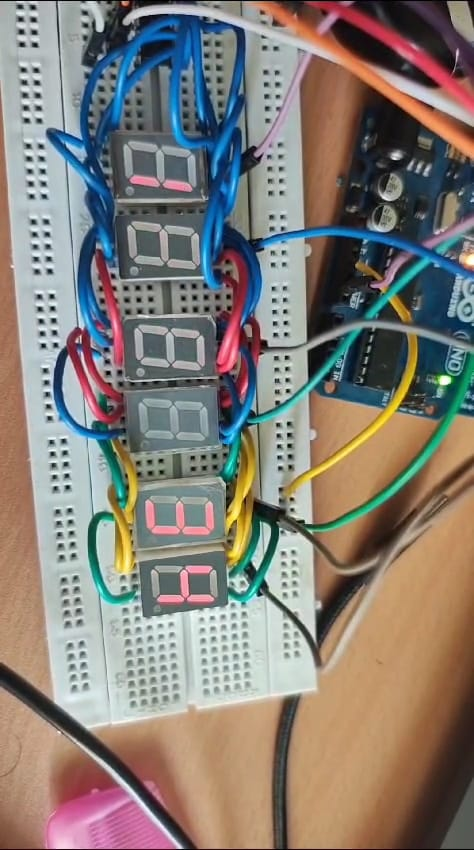
\includegraphics[width=0.35\linewidth]{WhatsApp Image 2025-03-24 at 18.30.23_1f184068.jpg}
    \caption{}
    \label{fig:enter-label}
\end{figure}